 \begin{surferPage}[Cayley-Kübik]{Cayley'nin Kübik Yüzeyi}
Bu kübik yüzey (\emph{üçgil}, yani derecesi $3$ olan yüzey) toplam dört adet çift koni tekilliğe sahip. $19$. yüzyılda kübikler konusunda çok araştırma yapmış olan Arthur Cayley'nin adıyla anılır.

Oysa  henüz 1863'te bu yüzeyleri üzerlerindeki olası tekilliklere göre  sistemli bir biçimde sınıflayan
Ludwig Schläfli idi. Örneğin bir kübik yüzey üzerinde niye $4$'ten fazla tekillik olamayacağı, makalesinde okunabilir. Böylece  $\mu(3)=4$ olduğunu biliyoruz.

1900 civarında  Felix Klein gerçel kübik yüzeylerin olası biçimleri üzerine çalışmıştır.
Fikri, Cayley'nin Kübik Yüzeyinden başlayarak ufak oynamalarla soruya cevap verebilmekti:
Çift koni tekilliklerini şişirerek, parçalayarak ya da bir araya getirerek  sonunda olası tüm biçimleri elde etti. Bunlardan birkaçı şöyle:
    \vspace{0.3cm}
     \begin{center}
      \vspace{-0.2cm}
      \begin{tabular}{@{}c@{\ }c@{\ }c@{\ }c@{}}
        \begin{tabular}{@{}c@{}}
          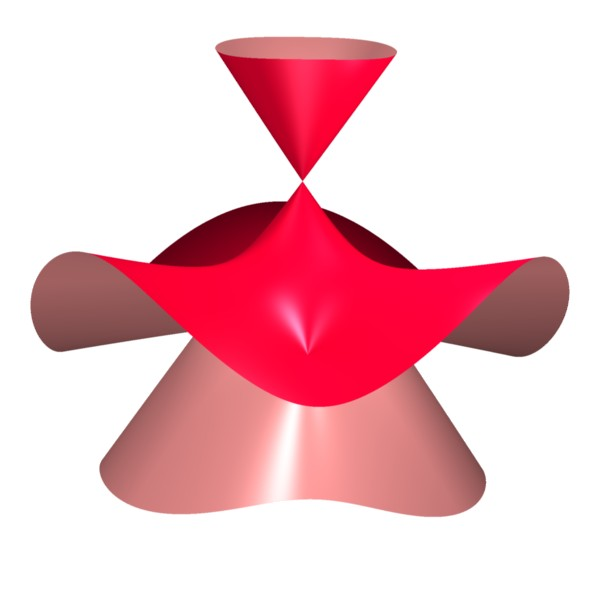
\includegraphics[width=1.35cm]{cayley_cubic_0}
        \end{tabular}
        &
        \begin{tabular}{@{}c@{}}
          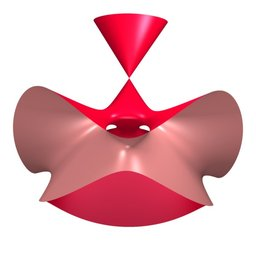
\includegraphics[width=1.35cm]{cayley_cubic_1}
        \end{tabular}
        &
        \begin{tabular}{@{}c@{}}
          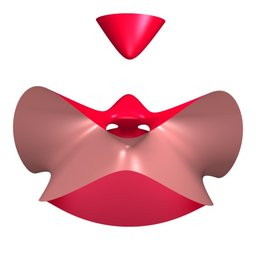
\includegraphics[width=1.35cm]{cayley_cubic_2}
        \end{tabular}
        &
        \begin{tabular}{@{}c@{}}
          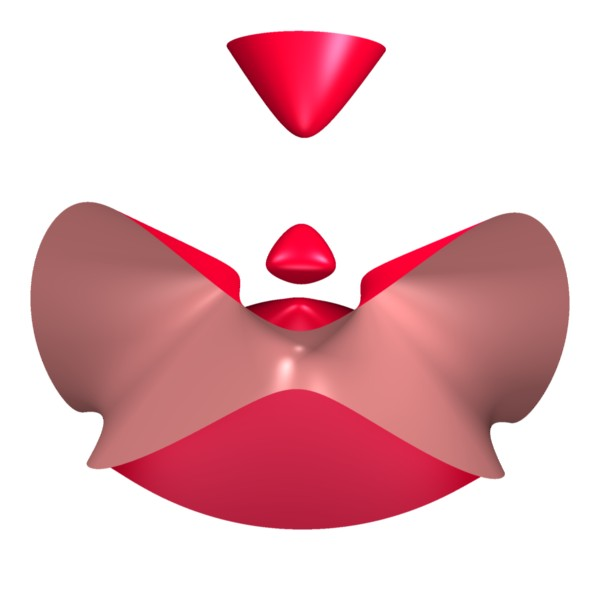
\includegraphics[width=1.35cm]{cayley_cubic_3}
        \end{tabular}
      \end{tabular}
    \end{center}
\end{surferPage}
